\documentclass{article}
\usepackage[margin=1in]{geometry}
\usepackage[linesnumbered,ruled,vlined]{algorithm2e}
\usepackage{amsfonts}
\usepackage{amsmath}
\usepackage{amssymb}
\usepackage{amsthm}
\usepackage{enumitem}
\usepackage{fancyhdr}
\usepackage{hyperref}
\usepackage{minted}
\usepackage{multicol}
\usepackage{pdfpages}
\usepackage{standalone}
\usepackage[many]{tcolorbox}
\usepackage{tikz-cd}
\usepackage{transparent}
\usepackage{xcolor}
% \tcbuselibrary{minted}

\author{Nathan Solomon}

\newcommand{\fig}[1]{
    \begin{center}
        \includegraphics[width=\textwidth]{#1}
    \end{center}
}

% Math commands
\renewcommand{\d}{\mathrm{d}}
\DeclareMathOperator{\id}{id}
\DeclareMathOperator{\im}{im}
\DeclareMathOperator{\proj}{proj}
\DeclareMathOperator{\Span}{span}
\DeclareMathOperator{\Tr}{Tr}
\DeclareMathOperator{\tr}{tr}
\DeclareMathOperator{\ad}{ad}
\DeclareMathOperator{\ord}{ord}
%%%%%%%%%%%%%%% \DeclareMathOperator{\sgn}{sgn}
\DeclareMathOperator{\Aut}{Aut}
\DeclareMathOperator{\Inn}{Inn}
\DeclareMathOperator{\Out}{Out}
\DeclareMathOperator{\stab}{stab}

\newcommand{\N}{\ensuremath{\mathbb{N}}}
\newcommand{\Z}{\ensuremath{\mathbb{Z}}}
\newcommand{\Q}{\ensuremath{\mathbb{Q}}}
\newcommand{\R}{\ensuremath{\mathbb{R}}}
\newcommand{\C}{\ensuremath{\mathbb{C}}}
\renewcommand{\H}{\ensuremath{\mathbb{H}}}
\newcommand{\F}{\ensuremath{\mathbb{F}}}

\newcommand{\E}{\ensuremath{\mathbb{E}}}
\renewcommand{\P}{\ensuremath{\mathbb{P}}}

\newcommand{\es}{\ensuremath{\varnothing}}
\newcommand{\inv}{\ensuremath{^{-1}}}
\newcommand{\eps}{\ensuremath{\varepsilon}}
\newcommand{\del}{\ensuremath{\partial}}
\renewcommand{\a}{\ensuremath{\alpha}}

\newcommand{\abs}[1]{\ensuremath{\left\lvert #1 \right\rvert}}
\newcommand{\norm}[1]{\ensuremath{\left\lVert #1\right\rVert}}
\newcommand{\mean}[1]{\ensuremath{\left\langle #1 \right\rangle}}
\newcommand{\floor}[1]{\ensuremath{\left\lfloor #1 \right\rfloor}}
\newcommand{\ceil}[1]{\ensuremath{\left\lceil #1 \right\rceil}}
\newcommand{\bra}[1]{\ensuremath{\left\langle #1 \right\rvert}}
\newcommand{\ket}[1]{\ensuremath{\left\lvert #1 \right\rangle}}
\newcommand{\braket}[2]{\ensuremath{\left.\left\langle #1\right\vert #2 \right\rangle}}

\newcommand{\catname}[1]{{\normalfont\textbf{#1}}}

\newcommand{\up}{\ensuremath{\uparrow}}
\newcommand{\down}{\ensuremath{\downarrow}}

% Custom environments
\newtheorem{thm}{Theorem}[section]

\definecolor{probBackgroundColor}{RGB}{250,240,240}
\definecolor{probAccentColor}{RGB}{140,40,0}
\newenvironment{prob}{
    \stepcounter{thm}
    \begin{tcolorbox}[
        boxrule=1pt,
        sharp corners,
        colback=probBackgroundColor,
        colframe=probAccentColor,
        borderline west={4pt}{0pt}{probAccentColor},
        breakable
    ]
    \color{probAccentColor}\textbf{Problem \thethm.} \color{black}
} {
    \end{tcolorbox}
}

\definecolor{exampleBackgroundColor}{RGB}{212,232,246}
\newenvironment{example}{
    \stepcounter{thm}
    \begin{tcolorbox}[
      boxrule=1pt,
      sharp corners,
      colback=exampleBackgroundColor,
      breakable
    ]
    \textbf{Example \thethm.}
} {
    \end{tcolorbox}
}

\definecolor{propBackgroundColor}{RGB}{255,245,220}
\definecolor{propAccentColor}{RGB}{150,100,0}
\newenvironment{prop}{
    \stepcounter{thm}
    \begin{tcolorbox}[
        boxrule=1pt,
        sharp corners,
        colback=propBackgroundColor,
        colframe=propAccentColor,
        breakable
    ]
    \color{propAccentColor}\textbf{Proposition \thethm. }\color{black}
} {
    \end{tcolorbox}
}

\definecolor{thmBackgroundColor}{RGB}{235,225,245}
\definecolor{thmAccentColor}{RGB}{50,0,100}
\renewenvironment{thm}{
    \stepcounter{thm}
    \begin{tcolorbox}[
        boxrule=1pt,
        sharp corners,
        colback=thmBackgroundColor,
        colframe=thmAccentColor,
        breakable
    ]
    \color{thmAccentColor}\textbf{Theorem \thethm. }\color{black}
} {
    \end{tcolorbox}
}

\definecolor{corBackgroundColor}{RGB}{240,250,250}
\definecolor{corAccentColor}{RGB}{50,100,100}
\newenvironment{cor}{
    \stepcounter{thm}
    \begin{tcolorbox}[
        enhanced,
        boxrule=0pt,
        frame hidden,
        sharp corners,
        colback=corBackgroundColor,
        borderline west={4pt}{0pt}{corAccentColor},
        breakable
    ]
    \color{corAccentColor}\textbf{Corollary \thethm. }\color{black}
} {
    \end{tcolorbox}
}

\definecolor{lemBackgroundColor}{RGB}{255,245,235}
\definecolor{lemAccentColor}{RGB}{250,125,0}
\newenvironment{lem}{
    \stepcounter{thm}
    \begin{tcolorbox}[
        enhanced,
        boxrule=0pt,
        frame hidden,
        sharp corners,
        colback=lemBackgroundColor,
        borderline west={4pt}{0pt}{lemAccentColor},
        breakable
    ]
    \color{lemAccentColor}\textbf{Lemma \thethm. }\color{black}
} {
    \end{tcolorbox}
}

\definecolor{proofBackgroundColor}{RGB}{255,255,255}
\definecolor{proofAccentColor}{RGB}{80,80,80}
\renewenvironment{proof}{
    \begin{tcolorbox}[
        enhanced,
        boxrule=1pt,
        sharp corners,
        colback=proofBackgroundColor,
        colframe=proofAccentColor,
        borderline west={4pt}{0pt}{proofAccentColor},
        breakable
    ]
    \color{proofAccentColor}\emph{\textbf{Proof. }}\color{black}
} {
    \qed \end{tcolorbox}
}

\definecolor{noteBackgroundColor}{RGB}{240,250,240}
\definecolor{noteAccentColor}{RGB}{30,130,30}
\newenvironment{note}{
    \begin{tcolorbox}[
        enhanced,
        boxrule=0pt,
        frame hidden,
        sharp corners,
        colback=noteBackgroundColor,
        borderline west={4pt}{0pt}{noteAccentColor},
        breakable
    ]
    \color{noteAccentColor}\textbf{Note. }\color{black}
} {
    \end{tcolorbox}
}


\fancyhf{}
\setlength{\headheight}{24pt}

\date{\today}
\title{Physics 127 Homework \#2}

\begin{document}
\maketitle

\begin{prob}
\end{prob}
\begin{enumerate}[label=(\alph*)]
    \item In the moving reference frame, the photon first moves from the bottom mirror to the top mirror along a line with speed $c$ and horizontal velocity $v$, so its vertical velocity is $\sqrt{c^2-v^2}=c/\gamma$. For the return trip, the photon moves from the top mirror to the bottom one with vertical velocity $-c/\gamma$, so the duration of the photon's round trip is $t'=2L\gamma/c$.
        \par
        In the lab frame, where the mirrors aren't moving, the horizontal velocity of the photon is also zero, so the duration of the round trip is $t=2L/c$. This is consistent with the time-dilation formula, $t'=\gamma t$.
    \item Once again, the round trip duration in the lab frame is $t=2L/c$. But in the moving frame, the right mirror is a distance of $L/\gamma$ from the left mirror, because of length contraction. The time it takes for the photon to move from the left mirror to the right mirror is $(L/\gamma)/(c-v)$, since the photon is moving to the right with speed $c$ and the right mirror is also moving to the right with speed $v$. For the same reason, the time it takes the photon to move from the right mirror to the left mirror is $(L/\gamma)/(c+v)$, so the duration of the round trip is
        \[ t' = \frac{L}{\gamma} \cdot \left( \frac{1}{c+v}+ \frac{1}{c-v} \right) = \frac{L}{\gamma} \cdot \frac{2c}{c^2-v^2} = \frac{2 \gamma L}{c}, \]
        which once again agrees with the formula $t'=\gamma t$.
\end{enumerate}

\bigskip
\par
\begin{prob}
    \textbf{Coleman problem 1.2:} A spaceship moves with velocity $v$ along its axis of symmetry. A star is at rest; the vector from the spaceship to the star makes an angle $\theta$ with this axis. What is the angle at which an observer on the spaceship sees the star?
\end{prob}
Suppose the spaceship is at the origin, moving in the $+x$ direction, and the star is a distance $L$ from the spaceship, at $(x=L\cos \theta, y=L\sin \theta)$.
\par
Then in the spaceship's reference frame, the horizontal lengths is contracted by a factor of $\gamma = 1/\sqrt{1-v^2/c^2}$, but the vertical length is the same. In this frame, the star's coordinates are $ (L \cos \theta \sqrt{1-v^2/c^2}, L \sin \theta)$. Therefore, the angle to the star is
\[ \theta' = \arctan \left( \frac{L \sin \theta}{L \cos \theta \sqrt{1-v^2/c^2}} \right) = \arctan \left( \frac{\tan\theta}{\sqrt{1 - \frac{v^2}{c^2}}} \right). \]

\bigskip
\par
\begin{prob}
\end{prob}
\begin{enumerate}[label=(\alph*)]
    \item The half-life in the $\pi$-meson's frame is $t=26 \si{.ns}$, so the half-life in the Earth's frame is
        \[ t = \gamma t = \frac{26\si{.ns}}{\sqrt{1-0.95^2}}\approx 83.3\si{.ns}. \]
    \item Since the speed is constant, average distance traveled is proportional to average time before decaying. We know the half-life is $\ln(2)$ times the expected lifetime, so the average distance traveled before decaying is
        \[ vt/\ln(2) = \frac{(0.95 c)(83.3 \si{.ns})}{\ln(2)} = 34.2 \si{.m}. \]
        
\end{enumerate}

\bigskip
\par
\begin{prob}
\end{prob}
\begin{enumerate}[label=(\alph*)]
    \item Using the definition of proper time,
        \[ v^i = \frac{\d x^i}{\d t} = \frac{\d x^i}{\d \tau} \cdot \frac{\d \tau}{\d t} = \frac{u^i}{\gamma}, \]
        so $u^\mu = \gamma v^\mu$, which means $u^0=\gamma$ and $u^i=\gamma v^i$ (for $i \in \{1,2,3\}$). Therefore $u \cdot u$ is
        \[ g_{\mu \nu} u^\mu u^\nu = \gamma^2 g_{\mu \nu} v^\mu v^\nu = \gamma^2 \left( 1 - v \cdot v \right) = 1. \]
        The derivative of the Lorentz factor with respect to proper time is
        \[ \frac{\d \gamma}{\d \tau} = \frac{\d}{\d \tau} (1-v^2)^{-1/2} = \left( - \frac{1}{2} (1-v^2)^{-3/2} \right) \left( -2v \right) \left( \frac{\d v}{\d \tau} \right) = \gamma^3 v \left( \frac{\d v}{\d t} \cdot \frac{\d t}{\d \tau} \right) = \gamma^4 v \cdot \dot{v}, \]
        so the 4-acceleration is
        \begin{align*}
        a^\mu &= \frac{\d u^\mu}{\d \tau} \\
              &= \frac{\d}{\d \tau} \left( \gamma, \gamma v^x, \gamma v^y, \gamma v^z \right) \\
              &= \left( \frac{\d \gamma}{\d \tau}, v^x \frac{\d \gamma}{\d \tau} + \gamma \frac{\d v^x}{\d \tau}, v^y \frac{\d \gamma}{\d \tau} + \gamma \frac{\d v^y}{\d \tau}, v^z \frac{\d \gamma}{\d \tau} + \gamma \frac{\d v^z}{\d \tau} \right) \\
              &= \left( \gamma^4 v \cdot \dot{v}, v^x \gamma^4 v \cdot \dot{v} + \gamma^2 \dot{v}^x, v^y \gamma^4 v \cdot \dot{v} + \gamma^2 \dot{v}^y, v^z \gamma^4 v \cdot \dot{v} + \gamma^2 \dot{v}^z \right) \\
              &= \left( \gamma^4 (v \cdot \dot{v}), v \gamma^4 (v \cdot \dot{v}) + \gamma^2 \dot{v} \right).
        \end{align*}
        The dot product $a \cdot u$ is
        \begin{align*}
        a\cdot u &= \left( \gamma^4 (v \cdot \dot{v}), v \gamma^4 (v \cdot \dot{v}) + \gamma^2 \dot{v} \right) \cdot \left( \gamma, \gamma v \right) \\
                 &= \gamma^5(v\cdot \dot{v}) - (\gamma v) \cdot (v \gamma^4(v \cdot \dot{v})+ \gamma^2 \dot{v}) \\
                 &= 0.
        \end{align*}
    \item The magnitude of $v^x$ is always less than 1, so the particle never reaches the speed of light.
        \par
        The components of the 4-velocity are
        \[ v^\mu = \begin{bmatrix}
            1 \\
            gt/\sqrt{1+g^2t^2} \\
            0 \\
            0
        \end{bmatrix}. \]
        The Lorentz factor is
        \[ \gamma = \frac{1}{\sqrt{1-(v^x)^2}} = 1+g^2t^2, \]
        therefore the proper time $\tau$ as a function of $t$ is
        \[ \tau = \int_{s=0}^{s=t} \frac{\d s}{\gamma(s)} = \int_{s=0}^{s=t} \frac{1}{1+g^2 s^2} \d s = \frac{\arctan(g t)}{g}. \]
        We can also write $t$ as a function of $\tau$ now:
        \[ t = \frac{\tan (g \tau)}{g}, \]
        which allows us to also write $x$ as a function of $\tau$:
        \[ x = \frac{gt}{\sqrt{1+g^2t^2}} = \frac{\tan^2 (g \tau)}{1+\tan^2(g\tau)} = \frac{\tan^2(g\tau)}{\sec^2 (g \tau)} = \sin^2(g\tau).\]
        
\end{enumerate}

\bigskip
\par
\begin{prob}
    Optional problem
\end{prob}
In the pole's reference frame, the doors are never simultaneously closed.

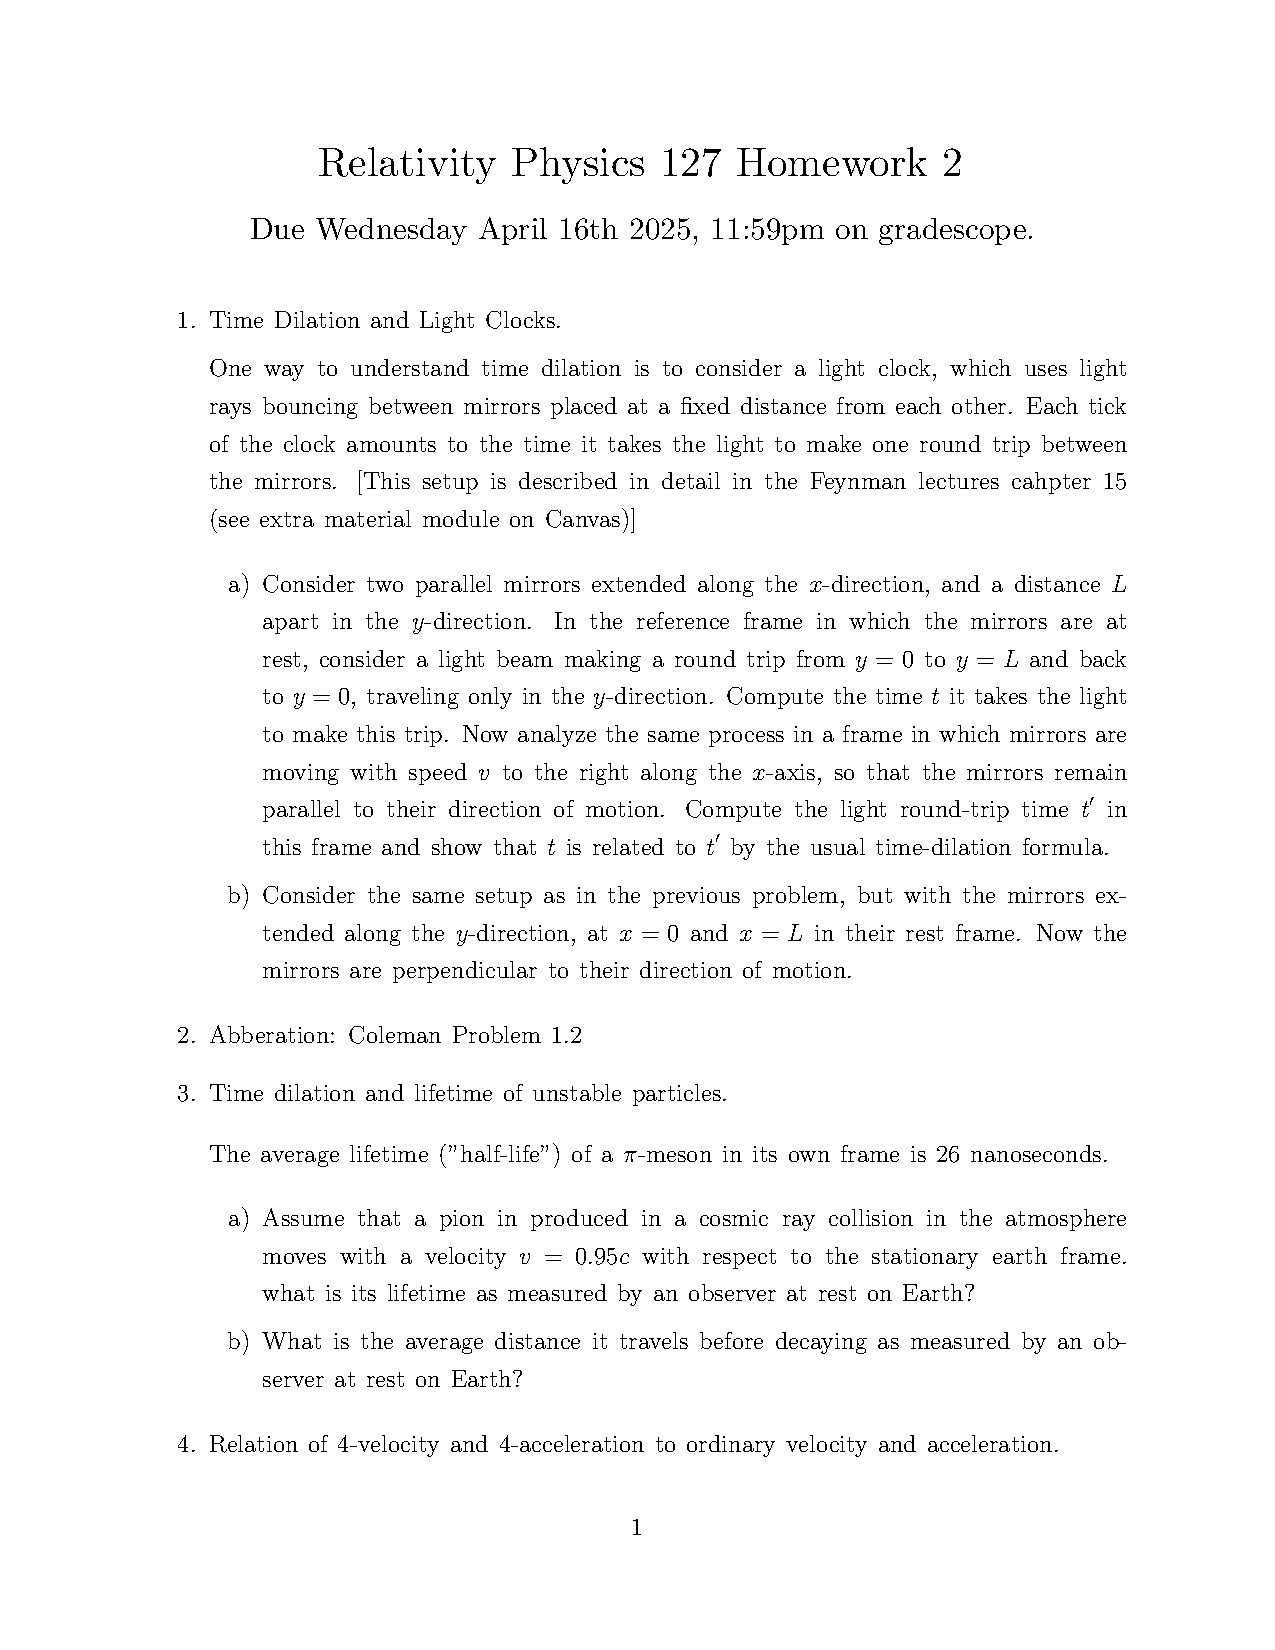
\includepdf[pages=-]{assignment.pdf}

\end{document}
